%  A simple AAU report template.
%  2015-05-08 v. 1.2.0
%  Copyright 2010-2015 by Jesper Kjær Nielsen <jkn@es.aau.dk>
%
%  This is free software: you can redistribute it and/or modify
%  it under the terms of the GNU General Public License as published by
%  the Free Software Foundation, either version 3 of the License, or
%  (at your option) any later version.
%
%  This is distributed in the hope that it will be useful,
%  but WITHOUT ANY WARRANTY; without even the implied warranty of
%  MERCHANTABILITY or FITNESS FOR A PARTICULAR PURPOSE.  See the
%  GNU General Public License for more details.
%
%  You can find the GNU General Public License at <http://www.gnu.org/licenses/>.
%
%  A simple AAU report template.
%  2015-05-08 v. 1.2.0
%  Copyright 2010-2015 by Jesper Kjær Nielsen <jkn@es.aau.dk>
%
%  This is free software: you can redistribute it and/or modify
%  it under the terms of the GNU General Public License as published by
%  the Free Software Foundation, either version 3 of the License, or
%  (at your option) any later version.
%
%  This is distributed in the hope that it will be useful,
%  but WITHOUT ANY WARRANTY; without even the implied warranty of
%  MERCHANTABILITY or FITNESS FOR A PARTICULAR PURPOSE.  See the
%  GNU General Public License for more details.
%
%  You can find the GNU General Public License at <http://www.gnu.org/licenses/>.
%
\documentclass[11pt,twoside,a4paper,openright]{article}
%%%%%%%%%%%%%%%%%%%%%%%%%%%%%%%%%%%%%%%%%%%%%%%%
% Language, Encoding and Fonts
% http://en.wikibooks.org/wiki/LaTeX/Internationalization
%%%%%%%%%%%%%%%%%%%%%%%%%%%%%%%%%%%%%%%%%%%%%%%%
% Select encoding of your inputs. Depends on
% your operating system and its default input
% encoding. Typically, you should use
%   Linux  : utf8 (most modern Linux distributions)
%            latin1 
%   Windows: ansinew
%            latin1 (works in most cases)
%   Mac    : applemac
% Notice that you can manually change the input
% encoding of your files by selecting "save as"
% an select the desired input encoding. 
\usepackage[utf8]{inputenc}
% Make latex understand and use the typographic
% rules of the language used in the document.
\usepackage[danish]{babel}
% Use the palatino font
\usepackage[sc]{mathpazo}
\linespread{1.05}         % Palatino needs more leading (space between lines)
% Choose the font encoding
\usepackage[T1]{fontenc}
%%%%%%%%%%%%%%%%%%%%%%%%%%%%%%%%%%%%%%%%%%%%%%%%
% Graphics and Tables
% http://en.wikibooks.org/wiki/LaTeX/Importing_Graphics
% http://en.wikibooks.org/wiki/LaTeX/Tables
% http://en.wikibooks.org/wiki/LaTeX/Colors
%%%%%%%%%%%%%%%%%%%%%%%%%%%%%%%%%%%%%%%%%%%%%%%%
% load a colour package
\usepackage{xcolor}
\definecolor{aaublue}{RGB}{33,26,82}% dark blue
% The standard graphics inclusion package
\usepackage{graphicx}
\graphicspath{{./grafik/}}
% Set up how figure and table captions are displayed
\usepackage{caption}
\captionsetup{%
  font=footnotesize,% set font size to footnotesize
  labelfont=bf % bold label (e.g., Figure 3.2) font
}
\usepackage{pdfpages}
\usepackage[numbers, sort&compress]{natbib}
% Make the standard latex tables look so much better
\usepackage{array,booktabs}
% Enable the use of frames around, e.g., theorems
% The framed package is used in the example environment
\usepackage{framed}
\usepackage[linewidth=2pt]{mdframed} %Bliver brugt til at lave en ramme om ting

%%%%%%%%%%%%%%%%%%%%%%%%%%%%%%%%%%%%%%%%%%%%%%%%
% Mathematics
% http://en.wikibooks.org/wiki/LaTeX/Mathematics
%%%%%%%%%%%%%%%%%%%%%%%%%%%%%%%%%%%%%%%%%%%%%%%%
% Defines new environments such as equation,
% align and split 
\usepackage{amsmath}
% Adds new math symbols
\usepackage{amssymb}
% Use theorems in your document
% The ntheorem package is also used for the example environment
% When using thmmarks, amsmath must be an option as well. Otherwise \eqref doesn't work anymore.
\usepackage[framed,amsmath,thmmarks]{ntheorem}

%%%%%%%%%%%%%%%%%%%%%%%%%%%%%%%%%%%%%%%%%%%%%%%%
% Page Layout
% http://en.wikibooks.org/wiki/LaTeX/Page_Layout
%%%%%%%%%%%%%%%%%%%%%%%%%%%%%%%%%%%%%%%%%%%%%%%%
% Change margins, papersize, etc of the document
\usepackage[
  inner=28mm,% left margin on an odd page
  outer=41mm,% right margin on an odd page
  ]{geometry}
% Modify how \chapter, \section, etc. look
% The titlesec package is very configureable
\usepackage{titlesec}
\titleformat{\chapter}[display]{\normalfont\huge\bfseries}{\chaptertitlename\ \thechapter}{20pt}{\Huge}
\titleformat*{\section}{\normalfont\Large\bfseries}
\titleformat*{\subsection}{\normalfont\large\bfseries}
\titleformat*{\subsubsection}{\normalfont\normalsize\bfseries}
%\titleformat*{\paragraph}{\normalfont\normalsize\bfseries}
%\titleformat*{\subparagraph}{\normalfont\normalsize\bfseries}

% Clear empty pages between chapters
\let\origdoublepage\cleardoublepage
\newcommand{\clearemptydoublepage}{%
  \clearpage
  {\pagestyle{empty}\origdoublepage}%
}
\let\cleardoublepage\clearemptydoublepage

% Change the headers and footers
\usepackage{fancyhdr}
\pagestyle{fancy}
\fancyhf{} %delete everything
\renewcommand{\headrulewidth}{0pt} %remove the horizontal line in the header
\fancyhead[RE]{\small\nouppercase\leftmark} %even page - chapter title
\fancyhead[LO]{\small\nouppercase\rightmark} %uneven page - section title
\fancyhead[LE,RO]{\thepage} %page number on all pages
% Do not stretch the content of a page. Instead,
% insert white space at the bottom of the page
\raggedbottom
% Enable arithmetics with length. Useful when
% typesetting the layout.
\usepackage{calc}

%%%%%%%%%%%%%%%%%%%%%%%%%%%%%%%%%%%%%%%%%%%%%%%%
% Bibliography
% http://en.wikibooks.org/wiki/LaTeX/Bibliography_Management
%%%%%%%%%%%%%%%%%%%%%%%%%%%%%%%%%%%%%%%%%%%%%%%%
%\usepackage[backend=bibtex,
%  bibencoding=utf8
%  ]{biblatex}
%\addbibresource{bib}

%%%%%%%%%%%%%%%%%%%%%%%%%%%%%%%%%%%%%%%%%%%%%%%%
% Misc
%%%%%%%%%%%%%%%%%%%%%%%%%%%%%%%%%%%%%%%%%%%%%%%%
% Add bibliography and index to the table of
% contents
\usepackage[nottoc]{tocbibind}
% Add the command \pageref{LastPage} which refers to the
% page number of the last page
\usepackage{lastpage}
% Add todo notes in the margin of the document
\usepackage[
%  disable, %turn off todonotes
  colorinlistoftodos, %enable a coloured square in the list of todos
  textwidth=\marginparwidth, %set the width of the todonotes
  textsize=scriptsize, %size of the text in the todonotes
  ]{todonotes}

%%%%%%%%%%%%%%%%%%%%%%%%%%%%%%%%%%%%%%%%%%%%%%%%
% Hyperlinks
% http://en.wikibooks.org/wiki/LaTeX/Hyperlinks
%%%%%%%%%%%%%%%%%%%%%%%%%%%%%%%%%%%%%%%%%%%%%%%%
% Enable hyperlinks and insert info into the pdf
% file. Hypperref should be loaded as one of the 
% last packages
\usepackage{hyperref}
\hypersetup{%
	pdfpagelabels=true,%
	plainpages=false,%
	pdfauthor={Author(s)},%
	pdftitle={Title},%
	pdfsubject={Subject},%
	bookmarksnumbered=true,%
	colorlinks=true,%
	citecolor=black,%
	filecolor=black,%
	linkcolor=black,% you should probably change this to black before printing
	urlcolor=black,%
	pdfstartview=FitH%
}

\usepackage{enumitem}
\usepackage{caption}
\usepackage{subcaption}
\usepackage[danish,nameinlink,capitalise]{cleveref}
\usepackage{listings}

\usepackage{tikz}
\usetikzlibrary{arrows}

% Additional commands
\newcommand{\namedtodo}[5]
{
  \ifthenelse{\equal{#1}{}}
  {
    \todo[backgroundcolor=#4,caption=
    {\textbf{#3: } #2}
    ,inline]
    {\color{#5}\textbf{#3: }#2}
  }
  {
    \todo[backgroundcolor=#4,caption=
    {\textbf{#3: } #1}
    ,inline]
    {\color{#5}\textbf{#3: }#2}
  }
}
\newcommand{\mikkel}[2][]{\namedtodo{#1}{#2}{Mikkel}{blue!80}{white}}
\newcommand{\stefan}[2][]{\namedtodo{#1}{#2}{Stefan M}{orange}{black}}
\newcommand{\mikael}[2][]{\namedtodo{#1}{#2}{Mikael}{green}{black}}
\newcommand{\bruno}[2][]{\namedtodo{#1}{#2}{Bruno}{black!10!red!90}{white}}
\newcommand{\lasse}[2][]{\namedtodo{#1}{#2}{Lasse}{black!10!yellow!90}{black}}
\newcommand{\als}[2][]{\namedtodo{#1}{#2}{Als}{purple!90!orange}{white}}
\newcommand{\winde}[2][]{\namedtodo{#1}{#2}{Winde}{black}{white}}
\newcommand{\lars}[2][]{\namedtodo{#1}{#2}{Lars}{blue!80}{black}}
\newcommand{\ivan}[2][]{\namedtodo{#1}{#2}{Ivan}{red}{black}}


  \makeatletter \renewcommand \listoftodos{\section*{List of Todos} \@starttoc{tdo}}
  \renewcommand\l@todo[2]
    {\par\noindent \textit{#2}, \parbox{10cm}{#1}\par} \makeatother
% Her er en liste over navnene på de forskellige styles
% C#: csharp
% F#: fsharp

% 
% Listings kan refereres vha. \cref{}
\crefname{listing}{code example}{code example}
\Crefname{listing}{Code example}{code examples}
% 

%Algoritmer i cref
\crefname{algocf}{algorithm}{algorithm}
\Crefname{algocf}{Algorithm}{Algorithms}
%Algoritmelinjer i cref
\crefalias{AlgoLine}{line}%

\makeatletter
\let\cref@old@stepcounter\stepcounter
\def\stepcounter#1{%
  \cref@old@stepcounter{#1}%
  \cref@constructprefix{#1}{\cref@result}%
  \@ifundefined{cref@#1@alias}%
    {\def\@tempa{#1}}%
    {\def\@tempa{\csname cref@#1@alias\endcsname}}%
  \protected@edef\cref@currentlabel{%
    [\@tempa][\arabic{#1}][\cref@result]%
    \csname p@#1\endcsname\csname the#1\endcsname}}
\makeatother
%

% Angivelse af navn på listings
\renewcommand\lstlistingname{Code example}
\renewcommand\lstlistlistingname{Code example}

\lstdefinestyle{standard}
{
	frame=shadowbox,
	framesep=5pt,
	rulecolor=\color{blue!40!black},
	rulesepcolor=\color{white!93!black},
	numbers=left,
	basicstyle=\ttfamily,
	numberstyle=\tiny,
	numberfirstline=true,
	%numberblanklines=false,
	stepnumber=1,
	numbersep=9pt,	
	captionpos=b,
	escapeinside={(*}{*)},
	breaklines=true,
	tabsize=4,
	language=c
}

\lstset{style=standard}

\lstdefinestyle{c}
{
	style=standard
}

\lstdefinestyle{csmall}
{
	style=c
}

\lstdefinestyle{csharp}
{
	style=standard,
	language=[Sharp]C
}
\lstdefinestyle{csharpsmall}
{
	style=csharp
}
\lstdefinestyle{fsharp}
{
	language=[Sharp]F,
	frame=lr,
	rulecolor=\color{blue!80!black}
}
\lstdefinestyle{fsharpsmall}
{
	style=fsharp,
	basicstyle=\ttfamily\footnotesize
}


% Definitions

% Superscript and subscript
\newcommand{\superscript}[1]{\ensuremath{^{\textrm{#1}}}}
\newcommand{\subscript}[1]{\ensuremath{_{\textrm{#1}}}}

% Degrees
\newcommand{\degree}{\ensuremath{^\circ}}
\newcommand{\dg}{\degree}

\newcommand{\quoter}[1]%
{
  \par
  \vspace{1.5em}
  \addtolength{\leftskip}{1.5cm}
  \addtolength{\rightskip}{1.5cm}
  \textit{#1}
  \addtolength{\leftskip}{-1.5cm}
  \addtolength{\rightskip}{-1.5cm}
  \vspace{1.5em}
  \par
}


\newcommand{\sensor}[3]
{
	\section{#1}
	#2
	
	#3
}

\newcommand{\analyse}[2]
{
\subsection{#1}
#2
}


% package inclusion and set up of the document
% see, e.g., http://en.wikibooks.org/wiki/LaTeX/Formatting#Hyphenation
% for more information on word hyphenation
\hyphenation{ex-am-ple hy-phen-a-tion short}
\hyphenation{long la-tex}
% 
%  A simple AAU report template.
%  2015-05-08 v. 1.2.0
%  Copyright 2010-2015 by Jesper Kjær Nielsen <jkn@es.aau.dk>
%
%  This is free software: you can redistribute it and/or modify
%  it under the terms of the GNU General Public License as published by
%  the Free Software Foundation, either version 3 of the License, or
%  (at your option) any later version.
%
%  This is distributed in the hope that it will be useful,
%  but WITHOUT ANY WARRANTY; without even the implied warranty of
%  MERCHANTABILITY or FITNESS FOR A PARTICULAR PURPOSE.  See the
%  GNU General Public License for more details.
%
%  You can find the GNU General Public License at <http://www.gnu.org/licenses/>.
%
%
%
% see, e.g., http://en.wikibooks.org/wiki/LaTeX/Customizing_LaTeX#New_commands
% for more information on how to create macros

%%%%%%%%%%%%%%%%%%%%%%%%%%%%%%%%%%%%%%%%%%%%%%%%
% Macros for the titlepage
%%%%%%%%%%%%%%%%%%%%%%%%%%%%%%%%%%%%%%%%%%%%%%%%
%Creates the aau titlepage
\newcommand{\aautitlepage}[3]{%
  {
    %set up various length
    \ifx\titlepageleftcolumnwidth\undefined
      \newlength{\titlepageleftcolumnwidth}
      \newlength{\titlepagerightcolumnwidth}
    \fi
    \setlength{\titlepageleftcolumnwidth}{0.5\textwidth-\tabcolsep}
    \setlength{\titlepagerightcolumnwidth}{\textwidth-2\tabcolsep-\titlepageleftcolumnwidth}
    %create title page
    \thispagestyle{empty}
    \noindent%
    \begin{tabular}{@{}ll@{}}
      \parbox{\titlepageleftcolumnwidth}{
        \iflanguage{danish}{%
          \includegraphics[width=.8\titlepageleftcolumnwidth]{aau_logo_da}
        }{%
          \includegraphics[width=.8\titlepageleftcolumnwidth]{aau_logo_en}
        }
      } &
      \parbox{\titlepagerightcolumnwidth}{\raggedleft\sf\small
        #2
      }\bigskip\\
       #1 &
      \parbox[t]{\titlepagerightcolumnwidth}{%
      \textbf{Abstract:}\bigskip\par
        \fbox{\parbox{\titlepagerightcolumnwidth-2\fboxsep-2\fboxrule}{%
          #3
        }}
      }\\
    \end{tabular}
    \vfill
    \iflanguage{danish}{%
      \noindent{\footnotesize\emph{Rapportens indhold er frit tilgængeligt, men offentliggørelse (med kildeangivelse) må kun ske efter aftale med forfatterne.}}
    }{%
      \noindent{\footnotesize\emph{The content of this report is freely available, but publication (with reference) may only be pursued due to agreement with the author.}}
    }
    \clearpage
  }
}

%Create english project info
\newcommand{\englishprojectinfo}[8]{%
  \parbox[t]{\titlepageleftcolumnwidth}{
    \textbf{Title:}\\ #1\bigskip\par
    \textbf{Theme:}\\ #2\bigskip\par
    \textbf{Project Period:}\\ #3\bigskip\par
    \textbf{Project Group:}\\ #4\bigskip\par
    \textbf{Participant(s):}\\ #5\bigskip\par
    \textbf{Supervisor(s):}\\ #6\bigskip\par
    \textbf{Copies:} #7\bigskip\par
    \textbf{Page Numbers:} \pageref{LastPage}\bigskip\par
    \textbf{Date of Completion:}\\ #8
  }
}

%Create danish project info
\newcommand{\danishprojectinfo}[8]{%
  \parbox[t]{\titlepageleftcolumnwidth}{
    \textbf{Titel:}\\ #1\medskip \par
    \textbf{Tema:}\\ #2\medskip \par
    \textbf{Projektperiode:}\\ #3\medskip \par
    \textbf{Projektgruppe:}\\ #4\medskip \par
    \textbf{Deltager(e):}\\ #5\medskip \par
    \textbf{Vejleder(e):}\\ #6\medskip \par
    \textbf{Oplagstal:} #7\medskip \par
    \textbf{Sidetal:} \pageref{LastPage}\medskip \par
    \textbf{Afleveringsdato:}\\ #8
  }
}

%%%%%%%%%%%%%%%%%%%%%%%%%%%%%%%%%%%%%%%%%%%%%%%%
% An example environment
%%%%%%%%%%%%%%%%%%%%%%%%%%%%%%%%%%%%%%%%%%%%%%%%
\theoremheaderfont{\normalfont\bfseries}
\theorembodyfont{\normalfont}
\theoremstyle{break}
\def\theoremframecommand{{\color{gray!50}\vrule width 5pt \hspace{5pt}}}
%\newshadedtheorem{exa}{Example}[chapter]
%\newenvironment{example}[1]{%
%		\begin{exa}[#1]
%}{%
%		\end{exa}
%}
% my new macros


\begin{document}
\begin{titlepage}



\begin{center}
\newcommand{\HRule}{\rule{\linewidth}{0.5mm}}
\HRule \\[0.4cm]
\Huge Entrepreneurship Miniprojekt A \\[0.3cm]

\HRule \\[1cm]
\noindent
  {\small
  Daníel Steínar Friðjónsson\\
  Lars Andersen\\
  Lasse Vang Gravesen\\
  Mathias Winde Pedersen\\
  Søren Skibsted Als\\}

\vfill
{\Large Entrepreneurship}
\\ ~\\
{\large Software 9. Semester, Aalborg Universitet, Efteråret 2015}

\end{center}
\end{titlepage}

\pagestyle{empty} %disable headers and footers
\pagenumbering{roman} %use roman page numbering in the frontmatter
%\hspace*{-1cm}\parbox[b][\textheight][t]{\textwidth}
{

\vspace{1cm}
\begin{center}
\textbf{\Huge {Software Innovation}} \\ \vspace{0.5cm}
\textbf{\Large Mini-projekt Type A}\\ \vspace{0.5cm}
\end{center}



\vspace{0.25cm}
\begin{center}
\item {\textbf{Deltagere:}} \\
Mikael Elkiær Christensen\\
Mikkel Sandø Larsen\\
Stefan Marstrand Getreuer Micheelsen\\
Bruno Thalmann\\
Søren Skibsted Als\\
Lars Andersen\\
Lasse Vang Gravesen\\
Mathias Winde Pedersen

\end{center}

\thispagestyle{empty}

\newpage
\thispagestyle{empty}
\mbox{}
}

\pagestyle{fancy} %enable headers and footers again
\setcounter{tocdepth}{1}
%\input{sections/preface.tex}
%mainmatter
\pagenumbering{arabic} %use arabic page numbering in the mainmatter

\section{Business Idea}
% The idea
The basic business idea for this miniproject is a Software as a Service product for webshops. 
The product itself is a recommender service, where the basic idea is to generate higher revenue for webshops by personalising product recommendations for their customers. 
The value proposition proposed is a core recommender system.
The webshop provide customer-product events to the company and the core recommender system builds a model based on this that can be used to return recommendations for specific customers.
The company then requests recommendations for specific customers, and are provided with model generated recommendations. 
The idea is then to access to the product through a subscription based license.
Additionally, consultancy services could be sold to install, maintain, customise and optimise the product. Furthermore, the consultancy services could be sold for other services in general.

% Resource-based Theory
To characterize and discuss this idea, we use Resource-based Theory based on \citet[pg. 13]{book:jrose}.
Resource-based theory is a theoretical concept where the idea is to describe what gives the company its competitive edge by looking at which resources and capabilities are available to it.
Resources included in this analysis of the company must be one of the following: Valuable, rare, costly to imitate, or non-substitutable.

The following resources are available to the company.
\begin{description}[style=nextline]
\item[Software Product]
The company provides a product that is valuable and expensive and difficult to replicate for webshops on their own. 
Additionally, we have a variety of possible algorithms that could be applied to different companies along with the core recommender system that can be adjusted per webshop.
\item[People \& Talent]
The company has software engineers with machine learning backgrounds and this is important for recommender systems. 
Additionally, there are very few machine learners in Denmark and as such these software engineers are rare. 
These software engineers can also be used for general machine learning consultancy jobs.
\item[Core Values]
The company aims to provide a high quality product, because we rely on our reputation to get and retain customers. 
If the product is low quality, customers would go elsewhere or not use it at all. 
\item[Knowledge]
The core competencies of the company lies within the domain of general machine learning applied to recommender systems. 
Additionally, the software engineers working for the company have a experience in business intelligence and general software development processes.
\item[Increased Capabilities]
Though it is intended that the core recommender system can be mostly used for any webshop, it can be adjusted and customised to the individual customer.
\end{description}

These resources lead to the following capabilities.
\begin{description}[style=nextline]
\item[Provide quality recommender systems]
Quality recommender systems have not yet been utilised to a great extent in Danish webshops.
\item[Improvement of knowledge base]
The field of recommender systems is still fairly young, and it being improved all the time. 
The company has the capability of improving general knowledge in regards to machine learning, recommender systems and business intelligence. 
Thereby the company can provide better value over time for the customers by iterative improvement of the value they receive through the recommender system by updating the core.
\item[Response to Customer Needs]
The company also has the capability of adjusting the model for a given customer, to improve their experience. This is done through a consultancy service.
\end{description}

These are overall valuable, rare, costly to imitate and non-substitutable which gives the company a competitive edge.

An alternative model to examine the business idea could have been the Five Forces model, where the threats to the company and its market are examined.
However, it was felt that there was no obvious threat at this point, as such the resource based theory seemed to fit better\citep[pg. 16]{book:jrose}.


%Describe your idea. Characterize and discuss it using at least one of the following models or theories (e.g. as part of sections on understanding, designing, or managing):
%Porter’s Value Chain
%Resource-based Theory
%Knowledge-based Theory
%Five Forces
%Change and Resistance Theory % Laska , larsks
\section{Business Model}
%Describe the most important elements in the canvas model for your idea
\begin{figure}
	\centering
	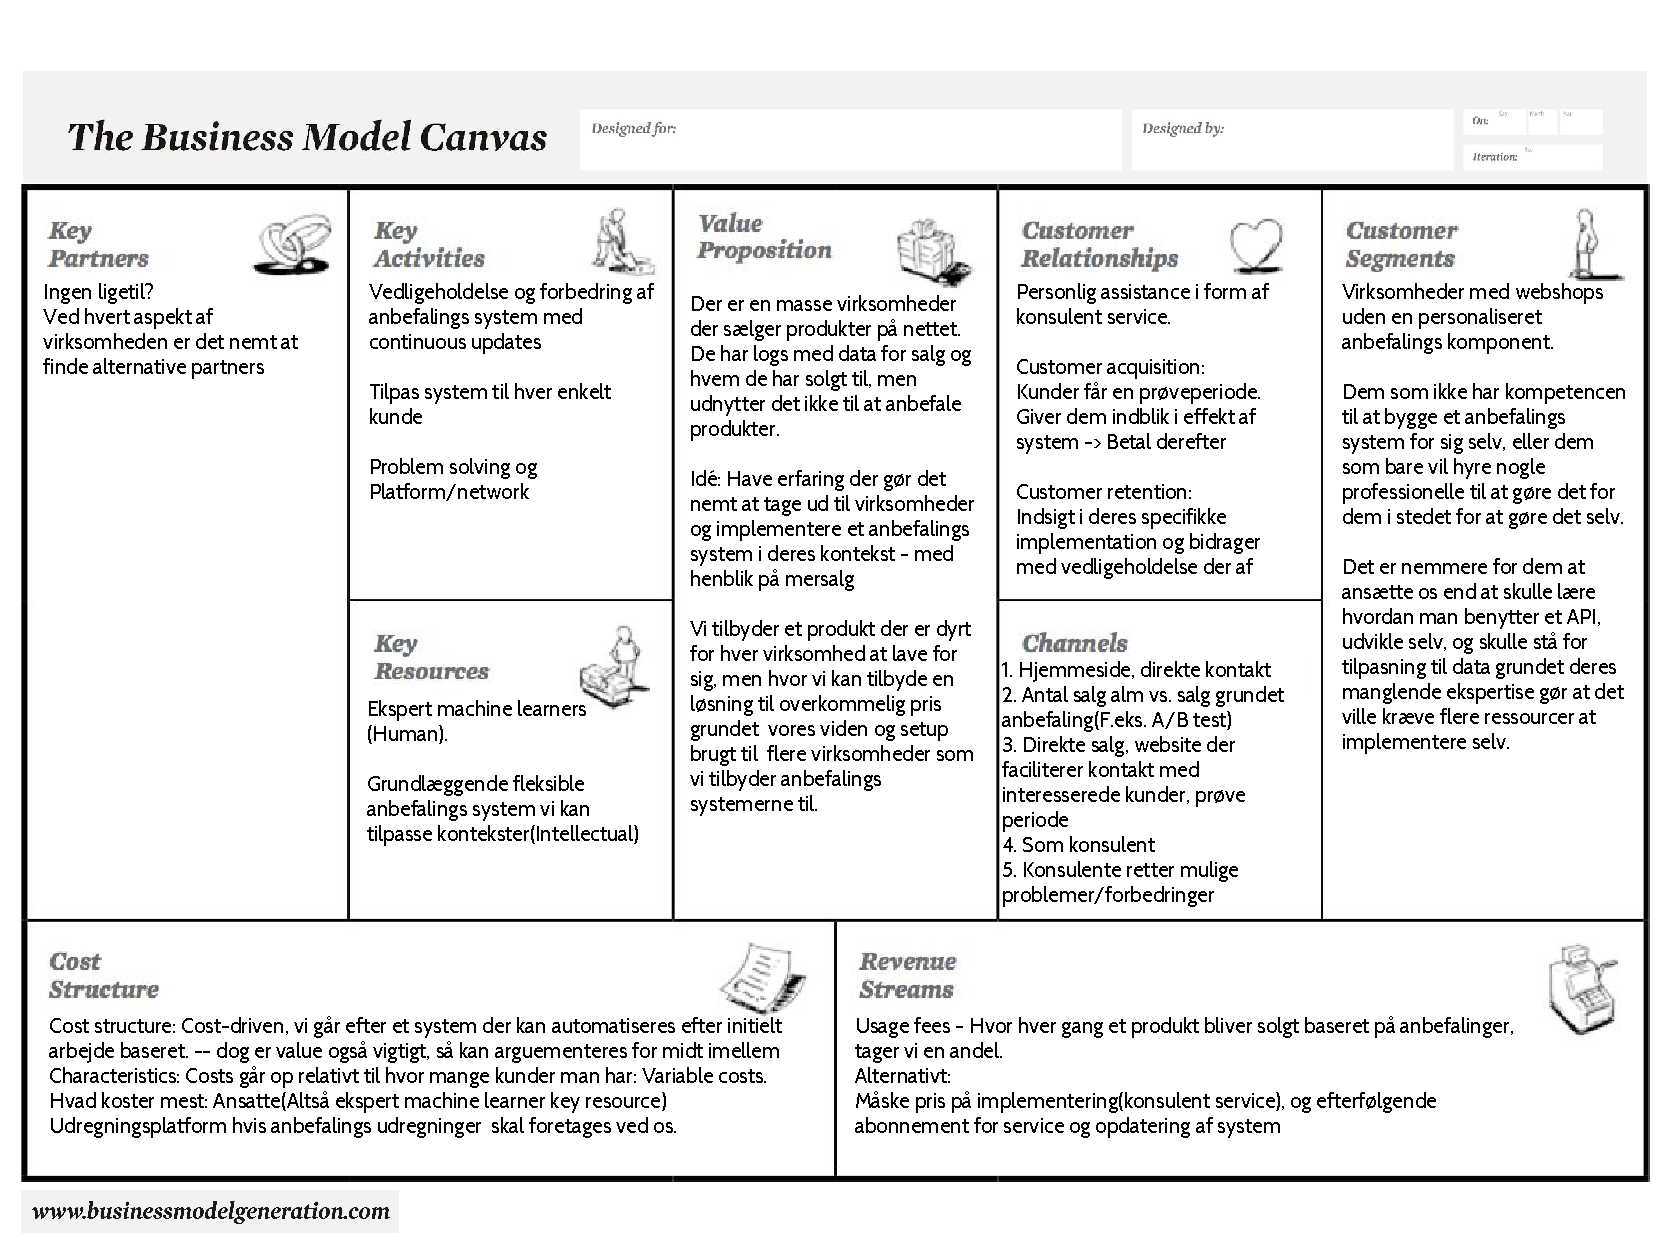
\includegraphics[width = 1.5\textwidth, angle=90]{figures/business-model-canvas}
	\caption{The Business Model Canvas for our Business Idea}
	\label{fig:BusinessModelCanvas}
\end{figure}

%    Describe your team under KR (key resources) - describe your technological expertise
The teams technological expertise lies within Machine Learning, which is where the overall idea comes from, given that product recommendation lies within the domain of machine Learning.

%    Characterize and discuss your VP (value proposition) and other relevant canvas elements using concepts from The software start-up chapter in the course notes (pages 40-55) and the e-Entrepreneurship chapter (pages 57-68)
In order to get an insight into the characteristics of the canvas elements, we answer a series of questions. 
The questions are from \citet[pg. 40-55]{book:jrose}.
The reason we need to answer these questions is because we see ourselves as arbitrageurs.
The arbitrageur exploits market inefficiencies, as there is very few companies that provide e-commerce solutions for local businesses. 
The other companies are typically too expensive for the small firms, and we strive to exploit this.
We exploit it by providing an customised and low-cost alternative.

\begin{description}[style=nextline]
	\item[Do  you  want  to  be  mainly  a  products  company  or  a  services  (consultancy)  company?] We see the product as SaaS(Software as a Service), with some additional optional consultancy work to customise the recommender solution to the webshops. For that reason it is a service company, where we have one core product.
	\item[Do  you  want  to  sell  to  individuals  or  enterprises,  or  to  mass  or  niche  markets?] The target audience of our product is enterprise companies and towards mass markets, as the product can be applied to virtually any webshop.
	\item[How  horizontal  (broad)  or  vertical  (specialized)  is  your  product  or  service?] Our service is vertical because of the scope of the business model. We have a very specialised product, the recommender system service, which we specialise in and strive to continuously improve.
	\item[Can  you  generate  a  recurring  revenue  stream  to  endure  in  good  times  and  bad?] Yes, since it is SaaS. In that way the customers pay a subscription fee to keep using the service.
	\item[Will  you  target  mainstream  customers,  or  do  you  have  a  plan  to  avoid  "the  chasm" - the gap between early adopters (the  rather  few  customers  with  specialised  interests  who  buy technically-innovative products),  and  the  early  majority  (the  many  customers  who  want  to buy  a  product  that  is  technically  sophisticated, but  also  established  and  popular)?] We target mainstream customers, and have no plans on targeting the early adopters or early majority types. In that way, we assume that the mainstream customers do not have the technical abilities to create their own recommender systems or want to invest their resources on developing their own. We think is a reasonable assumption due to the high lack of people with machine learning skills in Denmark.
	\item[Do  you  hope  to  be  a  leader  (a  company  that  is  an  innovator),  follower  (on  that basis  its products  on  established  technologies),  or  complementor  (a  company  that  provides additional  software  and  services  to  an  established  platform)?] We see ourselves as a complementor as we provide additional services that can improve the income of customers' webshop sales.
	\item[What  kind  of  character  (culture,  image,  brand,  working  environment)  do  you  want  your company  to  have?] We want our company to have a professional culture with an image that show that we are a disciplined company with high quality products and services.
\end{description}
Looking at the software business model, \citep[pg. 43]{book:jrose}, our company has a fairly high degree of involvement with the customers relationships, as we are consultants that can help businesses implement our solution. 
Additionally, the homogeneity of the product is also high, given that we want a standard backend that can be utilized in many different shops. 
As such we fit the ‘applied formats’, which means that we are offering a customizable solution based on a standard platform. One could also argue that it is software tailoring, since we customise the recommender system to the customers need, but what is tailored for each customer is only the parameters, e.g. their sales data and how to use it.

If we look at the software revenue generation model it can be characterised as SaaS.
We do, however, have a slight twist, since we use a free trial period.
Once the trial period is over though, the customer will be used to the increased sales that our system provides and sees no other option than paying us for a continuous use of the service.
In that way we can say that we use the bait \& hook pattern.

%    Discuss your canvas model. For example describe how it supports the implementation of your idea. Is it likely to change over time?
%    You may discuss pattern considerations (e.g. FREE or Open Business Models) using relevant concepts from the course notes
%    You may discuss your design approach (e.g. Customer Insights or Scenarios) using relevant concepts from the course notes
%    You may describe strategy concerns (e.g. Business Model Environment, Evaluation or Blue Ocean) using relevant concepts from the course notes

The canvas model gives a good representation of how we can bring our idea to life.
It describes the value proposition well, which is what part of the canvas that is least likely to change. 
However, as we get more customers, the solution may become less customised to each firm we provide a service to, and more of a standardised solution.

One could imagine that depending on the customers we are in contact with, the revenue stream may change. 
An alternative to the subscription based solution is to make an agreement with the company that we gain a part of the profit from the increased sales that the recommender system provides.
Such a change may be interesting for webshops we believe have an extreme growth potential.

For the other parts of the business canvas model, we cannot at this point in time imagine what may change. 
However, one of the advantages of the business canvas model is that it gives a short outline of the business model that can be changed if necessary as we experience change in our entrepreneurial process.

\subsection{Storytelling}
To gain a better outlook of the business idea, and to illustrate how we utilise the bait \& hook pattern, we drew a storyboard, which can be seen in Figure \cref{fig:drawing}.

\begin{figure}
	\centering
	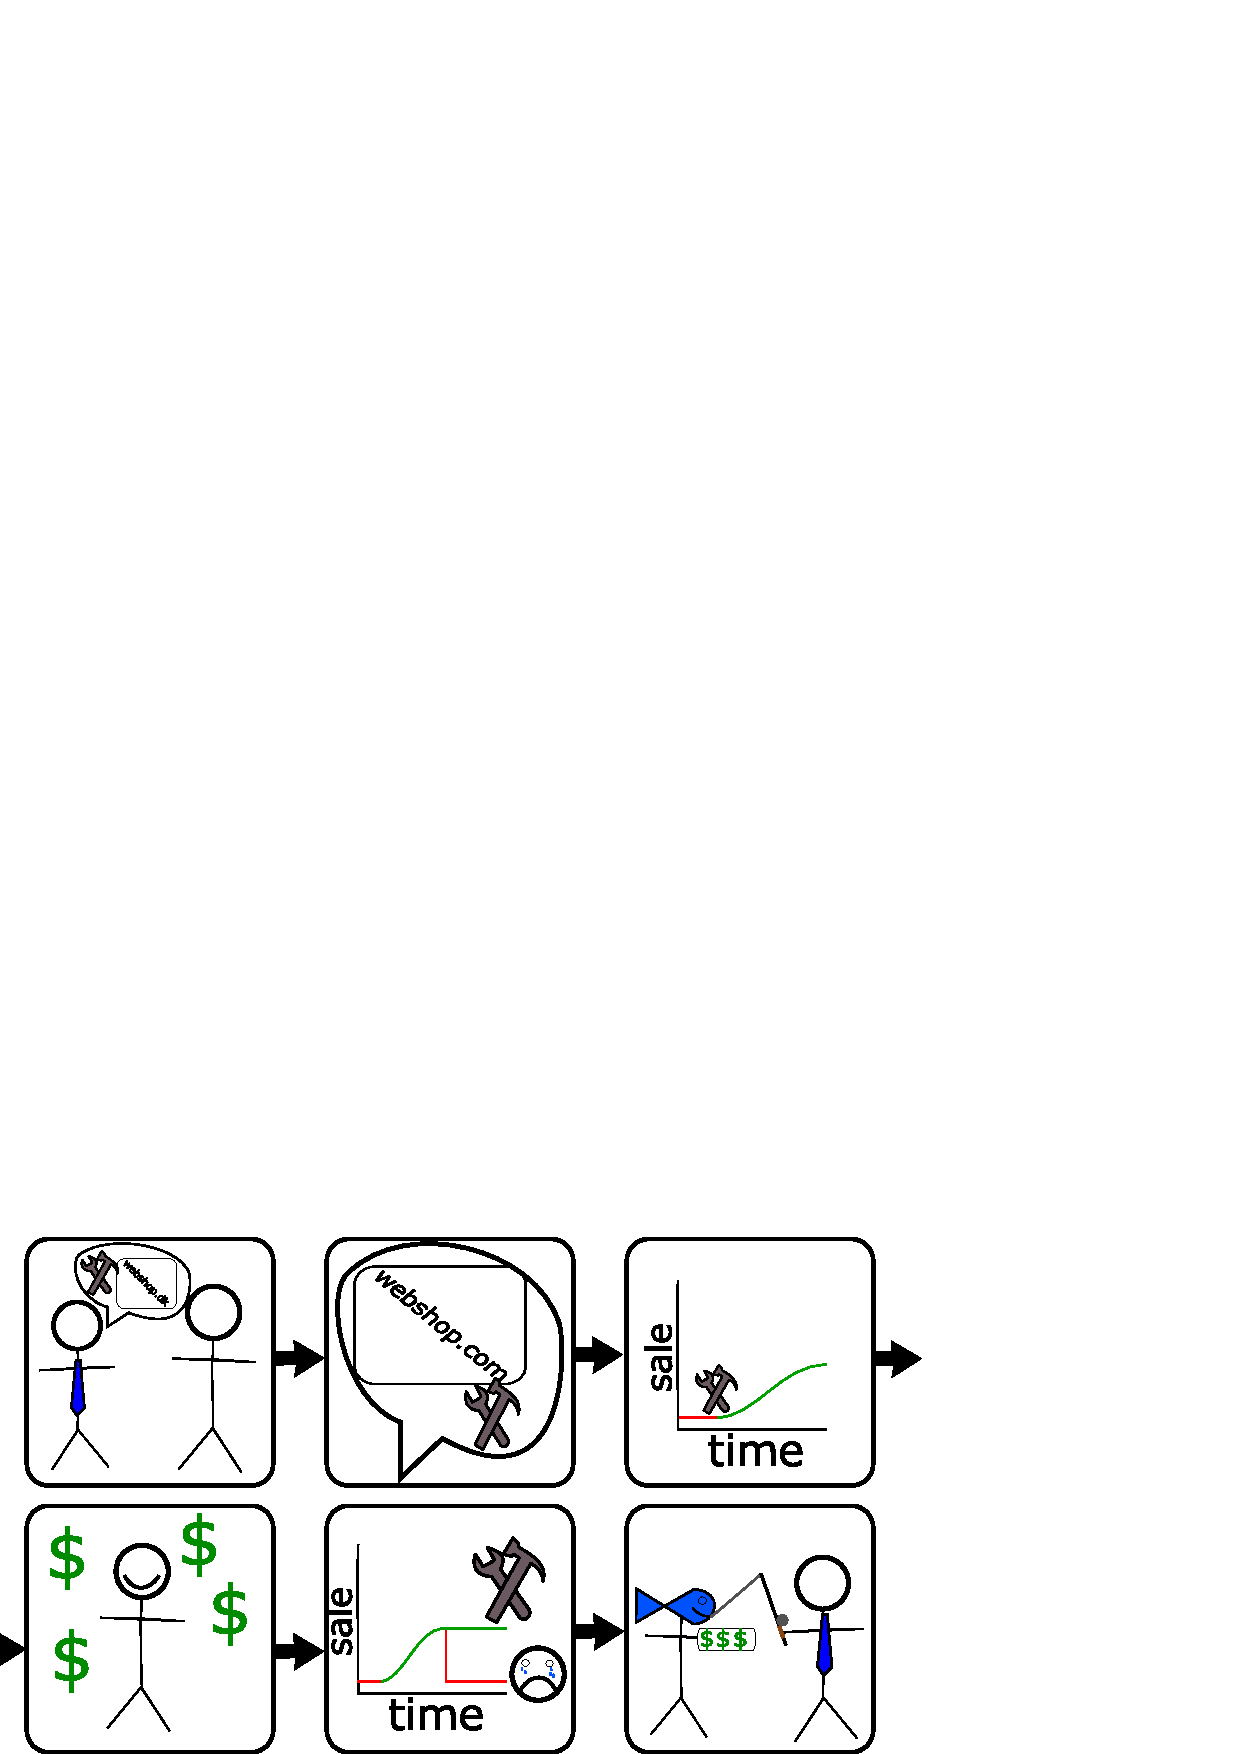
\includegraphics[width=0.7\linewidth]{figures/drawing}
	\caption{Story board of how we use the bait \& hook pattern.}
	\label{fig:drawing}
\end{figure}
 
 On frame one and two we introduce our recommender system solution to the customer who owns a webshop.
 Frame 3 and 4 shows how the customer becomes happy since our solution increased his sales in the trial period he got.
 However, when we come to frame 5 the customer becomes unhappy if he stops paying, since his sales will then drop again.
 Finally on frame 6 we show how the customer has then turned into a fish that we catch, i.e. we have hooked him and he has to keep paying to keep the increased sales on his webshop.
 
\subsection{Strategy Concerns}
To identify the strategy concerns we use the questions from \citet[pg. 202-208]{osterwalder2010business}.
The concerns we find most important is answered hereafter.

One of the strategies we find interesting was the market issues which identifies key issues that can drive and transform our market from customer and offer perspective.
\begin{description}[style=nextline]
	\item[What are the crucial issues affecting the customer landscape?] It is very important for the retailers that are our customers to sell as much as possible in their shops, and to retain their customers and keep the customers engaged.
	\item[Where is the market heading?] The market seems fairly stagnant, with recommender systems only being made in-house. However, in recent years Business Intelligence and big data has become an area of large interest, wherein we identify recommender systems a part of.
\end{description}

Another part we find interesting is the questions regarding the market segment.
\begin{description}[style=nextline]
	\item[What are the most important Customer Segments?] Webshops and retailers that could benefit from increased sales from recommender systems.
	\item[Where is the biggest growth potential?] In case we can obtain a good contract with large web shops, a larger profit can be obtained. The regular subscription fee will be sufficient to keep the company alive though. That is, the percentage based approach has the potential for more growth, but also requires us to score better customers than if it just a regular subscription fee they pay.
	\item[Which peripheral segments deserve attention?] Websites such as GoodReads, but ones that do not have their own recommender systems made in-house or ones with recommender systems that we can beat (catalog websites). Other solutions where recommendations can be useful, in ways similar to netflix, libraries etc. where users consume information content.
\end{description}

It is also important to discuss the switching cost questions.
\begin{description}[style=nextline]
	\item[What binds customers to a company and its offer?] Bait and hook: They see the increased sales that the recommender system gave them, and have to keep paying to keep the increased sales.
	\item[What switching costs prevent customers from defecting to competitors?] Implementation of the recommender system in their own site, and needing to either pay the competitors to implement it or paying on their own. Also, a risk of getting a lower quality service if swapping to competitors.
	\item[How important is brand?] It is important, as our motto is: “We increase sales”. On the other hand, it is not represented on the site that we delivered the recommender system too. Therefore, it just needs to work, there is no prestige in using a specific recommender system.
\end{description}


In recent times there has been a huge technological interest in webshops, recommender systems and the like. For that reason we present answers to some technological aspects.
\begin{description}[style=nextline]
	\item[What are the major technology trends both inside and outside your market?] New methods for recommender systems are always coming up, and it is a technology that has not fully matured yet and will continue to improve over time. Web shops are getting easier and easier to implement without expertise.
	\item[Which technologies represent important opportunities or disruptive threats?] Web shops that make it easy to implement recommender systems without requiring expertise. Another threat could be templates for webshops, where a recommender system is included as part of the template. 
\end{description}

There has been a shift in recent years, where the population has gone more online.
This shift makes it relevant to answer the following questions.
\begin{description}[style=nextline]
	\item[Describe key societal trends:] A lot of businesses are moving online to the internet and this can help us.
	\item[Which shifts in cultural or societal values affect your business model?] Moving internet businesses off of the internet and into the real world, but this is unlikely.
	\item[Which trends might influence buyer behavior?] Deciding not to get a web shop but instead use a real world shop. Might be likely for people with no technological expertise or knowhow on how to do this.
\end{description} %windka, danka, sòrka
\section{Paradigm}
In this section, we discuss, choose and outline how to apply one of the two paradigms for software entrepreneurship.

There are two paradigms to choose from as specified in \citet[pg. 30-32]{book:jrose}: Analyse, Design, Enact (ADE) and Consider, Do, Adjust (CDA). 
We choose the Consider, Do, Adjust paradigm, where the model is a modified version called the Build-Measure-Learn loop from \citet[pg. 75]{ries2011lean}. 
The Build-Measure-Learn feedback loop starts with an idea that inspires building a minimum viable product.
Once a product has been built, the idea is to measure available data and to learn from the experience.
The goal of the model is to minimize the total time through the loop. 

That is entering the Build phase, the first recommender system is the minimum viable product (MVP) introduced in The Lean Startup, \citep[pg. 77]{ries2011lean}.
This MVP version of the product enables a full turn in the Build-Measure-Learn loop with a minimum amount of effort, because this MVP is generally lacking in comparison to the SaaS solution that is intended to be the final product.
In the Measure phase, the company needs to determine if the product being developed has any appeal to the intended customers. 
One way to measure is through a concept called 'Innovation Accounting'\citep[pg. 77]{ries2011lean}.
'Innovation Accounting' is a quantitative approach that allows seeing if the efforts are bearing fruit and allows the company to create learning milistones. 
Finally, entering the Learn phase of the Build-Measure-Learn loop the company must ask itself whether to pivot or persevere with the original strategy.
That is, change the direction of the company or stay the course. 

As such we think, the approach should be as follows:

First of all a single webshop is contacted and offered a custom made recommender solution. 
This is done because developing such a recommender system will help us gain experience and give us ideas on how to proceed on how to create a Software-as-a-Service product that can be generalised to other webshops.
We then enter the Measure phase, we measure the we gain customers as we build custom made recommender systems with the goal of eventually creating a core recommender system that can be used as SaaS.
In the Learn loop, we will decide if we want to pivot or persevere. Eventually, we will have built enough experience to take advantage of the fact that all the recommender systems are similar and can be generalised into a core recommender system that can be used as SaaS.
This will in turn make the maintainability of the recommender systems easier, giving the company the opportunity to provide recommender systems to more companies without losing overview. 

% Outline important financial concerns for your project relative to the choice of paradigm.
Additionally, our choice of paradigm creates financial concerns. 
Given the Build-Measure-Learn loop described, the primary financial concern for the company is to ensure that there is revenue generation during the loops before the core recommender system can be established. 
Specifically, paying wages is a primary financial concern with no steady income from the subscription based license. 
Additionally, there is the concern that it is unknown how long a basic recommender system will take to build to our quality standards, even for a MVP.
It might become a problem if the MVP takes too long for the webshop to be built and they do not want to pay for the time it takes to build.

% Outline phases or activities in the Business Model Design Process.
In \citet[pg. 241-261]{osterwalder2010business}, The Business Model Design Process has 5 different phases: Mobilize, Understand, Design, Implement and Manage.
The Mobilize phase is where the preparation for the design process is done.
What we did for this phase was decide to use a Business Model Canvas based on the initial idea.

The Understand phase is where elements for the design effort are researched and analysed. 
What we did for this phase was identify possible customers, use storytelling to gain clarity about the business idea and how it should function.

The Design phase is where business models are generated, tested and selected.
What we did for this phase was create a business model canvas.

The first three steps alone are the idea part of the Build-Measure-Learn loop, that and what comes after is the Building of the MVP, Measuring the effect, and Learning from it and possibly pivoting or staying the course. 
As such the Implement phase, where the business model is implemented in the field is the Build phase.
The Manage phase, where the business model is adapted or modified in response to the market reaction are then the Measure and Learn parts of the loop.

Obviously the Build-Measure-Learn loop is more conducive to an approach that spends little time in research and instead spends more time on creating a MVP that can be used to launch the business quickly, measuring the effect and learning from it and seeing what should be changed.

%Discuss, choose, and outline how to apply one of the two paradigms for software entrepreneurship
%
%Analyse, Design, Enact (ADE)
%Consider, Do, Adjust (CDA)
%Outline phases or activities in the Business Model Design Process
%Outline important financial concerns for your project relative to the choice of paradigm
\section{Project Theory}
In the papers, \citet{Sarasvathy2003203} and \citet{sarasvathy2001causation}, Sarasvathy discusses causation, effectuation the link to near decomposability.
The logic of causation is defining the market, segmenting the customers, targeting the customers and positioning in the market all to reach the customer. 
That is given a particular goal I want to achieve, what ought I to do and what particular path should I take.
Inversely, effectuation is rather looking at the means available and determining what could be done.
Effectuation also assumes that the future is controllable such that we can reduce the need to predict uncertain future events.
The difference between causation and effectuation can be visualised in \cref{fig:causation_effectuation}.
Saravathy's effectuation model was primarily targeted towards the suicide quadrant where the markets and products are new and predictability is low.

\begin{figure}
	\centering
	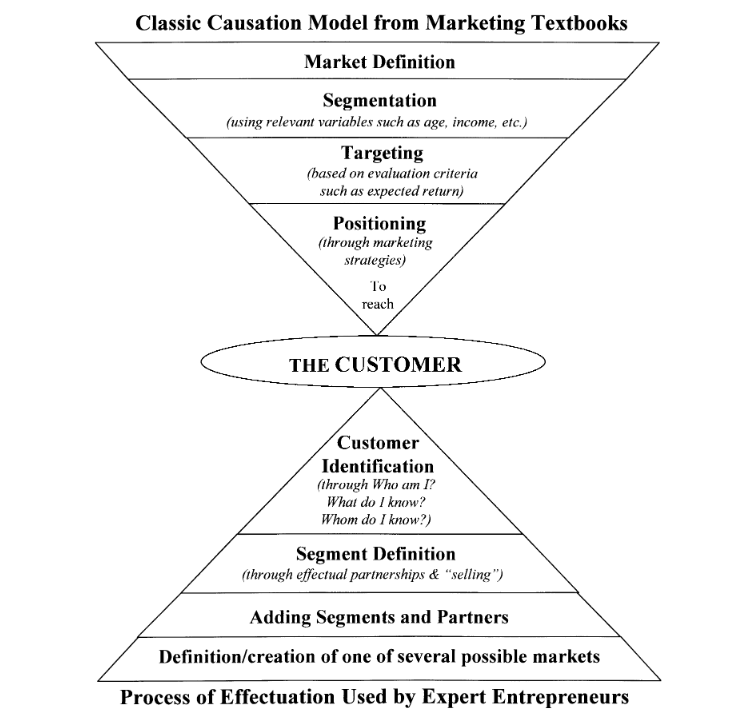
\includegraphics[scale=0.3]{causation_effectuation_pyramid}
	\caption{Effectual contrasting causation from \citet{Sarasvathy2003203}}
	\label{fig:causation_effectuation}
\end{figure}

Causation in relation to this project is the fact that the goal was approached first, and as a result of the goal the rest were examined. 
Effectuation could, however, also be argued for in the sense that the means of the group were examined as a result of that different ideas were examined.
                                                                                                              
In near-decomposable systems the behaviour of components are approximately independent of other components and this creates the effect that systems that are near-decomposable have a higher chance of succeeding in the sense that even if one component in the system fails the entire system will not fail.
We do not believe that our business is near-decomposable, because if it fails gain a market it is necessary to pivot onto a different idea or a different market \citep[pg. 149-178]{ries2011lean}.
But in the case that our customers go bankrupt the company is not severely affected outside of the loss of the subscription license fee. 
In addition, a lot of webshops exists so it should be easy to find other webshops to pay a subscription fee.


\citet{doi:10.1108/S1876-0228(2012)0000009015} challenges the idea of effectuation only being useful in the suicide quadrant and instead that it can be used in other combinations as well.
Kraaijenbrink states that causation and effectuation should be seen as two extremes and it is more beneficial to look at the dimension values that define these models.
As of such the dimensions of these models can be chosen to one's needs, and thus creating a model depending on the market and product.
The dimensions can be seen in \cref{fig:kraaijenbrink}.

The characteristics of our entrepreneurial behaviour are as such:
\begin{description}
	\item[Means-driven vs. Ends-Driven] Means-driven as we have knowledge and experience with recommender systems and try to make a business based on these means.
	\item[Control vs. Prediction] Arguably we have some predictability. That is, we foresee that the e-commerce genre is steadily increasing, and for that reason we believe there is going to be a high demand for high quality recommender systems. The predictability of the business model means it lies outside of the suicide quadrant.
	When it comes to control we cannot pinpoint any specific aspects we can control, one way to control is if we partner with some stakeholder that can affect/control the future in some way, since a lot of the future is affected by human actions/behaviour.
	\item[Affordable loss vs. Expected returns] It is affordable loss since development time is primarily invested for such a business, there is not really any expensive equipment etc. that should be bought. One example of a loss could be if some high tech server is invested in, but for the MVP it is not necessary.
	\item[New products and markets vs. existing products and markets] The product could be either existing or new, in the sense that it could be rationalised as either because the idea of a recommender system is not new but the product itself is new. 
	It is a new market because recommender systems delivered by a third party is not common in Denmark. Something similar exists for a company such as the Hut Group, which is a company that owns over 100 webshops, where they have a centralised backend including recommender systems. That is a company that owns a large amount webshops though, and is not really the market we are targeting, as we are instead targeting webshops where they lack experience or resources to develop a recommender system themselves.
	\item[Cooperation vs. Competition] Cooperation is in focus, as it of utmost importance to gain confidence with the webshops we deliver recommender systems to. We both benefit from the increased sales the recommender system will give.
	\item[Cyclical vs. Linear] Cyclical, we do not indulge in a linear process. That is, we believe the consider-do-adjust paradigm is beneficial, and also follow it since we want to utilise the Lean Startup Build-Measure-Learn loop \citep[pg. 75]{ries2011lean}.
\end{description}

\begin{figure}[!htb]
	\centering
	\includegraphics[scale=0.4]{kraaijenbrink}
	\caption{Human action and entrepreneurial behaviour from \citet{doi:10.1108/S1876-0228(2012)0000009015}}
	\label{fig:kraaijenbrink}
\end{figure}

%Discuss your project theoretically using at least two papers from the syllabus
%
%    Is your choice of paradigm theoretically or empirically justifiable? In what way?
%    Relate your project to concepts from syllabus papers; e.g. effectuation/causation principles✓ , predictability,✓  problem spaces (e.g. suicide quadrant),✓  marketing, lean development, or software development practices.

 

\bibliographystyle{unsrtnat}
\bibliography{bib}
\label{bib:mybiblio}

\appendix
%\input{dogmeregler}

\end{document}
